\documentclass[12pt]{article}
\usepackage[utf8]{inputenc}
\usepackage[T1]{fontenc}
\usepackage[catalan]{babel}
\usepackage{amsmath, amssymb, amsfonts}
\usepackage{geometry}
\usepackage{fancyhdr}
\usepackage{graphicx}
\usepackage{tikz}
\usetikzlibrary{matrix, calc, arrows.meta}
\usepackage{tcolorbox}
\usepackage[colorlinks=true, linkcolor=blue]{hyperref}
\usepackage{float}
\usepackage{enumitem}
\usepackage{tabularx}
\usepackage{booktabs}
\usepackage{array}

\setlength{\headheight}{16pt}
\geometry{a4paper, left=2cm, right=2cm, top=2.5cm, bottom=2.5cm}

\pagestyle{fancy}
\fancyhf{}
\fancyhead[L]{MACS 1r Batxillerat}
\fancyhead[R]{\leftmark}
\fancyfoot[L]{\href{mailto:oscar.rodriguez@insjoseplladonosa.cat}{oscar.rodriguez@insjoseplladonosa.cat}}
\fancyfoot[R]{\thepage}

% Entorns personalitzats
\newtcolorbox{concept}[1][]{colback=blue!5!white, colframe=blue!75!black, fonttitle=\bfseries, title=Concepte, #1}
\newtcolorbox{exemple}[1][]{colback=green!5!white, colframe=green!75!black, fonttitle=\bfseries, title=Exemple, #1}
\newtcolorbox{exercici}[1][]{colback=yellow!10!white, colframe=yellow!75!black, fonttitle=\bfseries, title=Exercici, #1}
\newtcolorbox{solucio}[1][]{colback=orange!5!white, colframe=orange!75!black, fonttitle=\bfseries, title=Solució, #1}
\newtcolorbox{resum}[1][]{colback=purple!5!white, colframe=purple!75!black, fonttitle=\bfseries, title=Resum de fórmules, #1}

\hypersetup{pageanchor=false}
\begin{document}

\begin{titlepage}
    \centering
    \vspace*{0.5cm}
    {\Large \textbf{INS Josep Lladonosa} \par}
    \vspace{0.3cm}
    {\large Matemàtiques Aplicades a les Ciències Socials -- 1r de Batxillerat \par}
    \vspace{1.5cm}
    {\Huge \textbf{Tema 2: Els Polinomis} \par}
    \vspace{0.8cm}
    {\Large Dossier de Teoria i Exercicis \par}
    \vspace{1.5cm}

    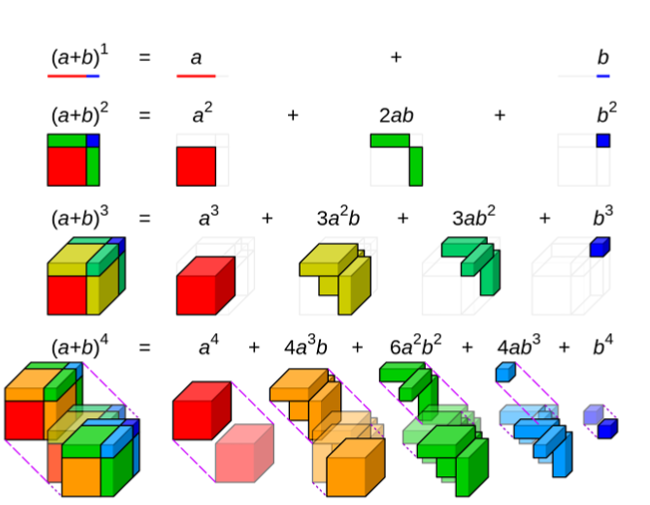
\includegraphics[width=0.55\textwidth]{polinomis.png}

    \vspace{1.5cm}
    \textbf{Professor:} Òscar Rodríguez \\
    \href{mailto:oscar.rodriguez@insjoseplladonosa.cat}{oscar.rodriguez@insjoseplladonosa.cat}
\end{titlepage}

\tableofcontents
\newpage

\hypersetup{pageanchor=true}
\pagenumbering{arabic}

% =========================================================
\section{Monomis}

% ---------------------------------------------------------
\subsection{Definició i elements}

\begin{concept}
\textbf{Definició de monomi}\\
Un \textbf{monomi} és una expressió algebraica formada pel producte d'un nombre real, anomenat \textbf{coeficient}, i una o més variables o incògnites que constitueixen la \textbf{part literal}. Cada variable té el seu exponent, i la suma de tots els exponents s'anomena \textbf{grau del monomi}.

\textbf{Elements:}
\begin{itemize}
    \item \textbf{Coeficient:} el nombre que multiplica la part literal.
    \item \textbf{Part literal:} el producte de les variables amb els seus exponents.
    \item \textbf{Grau:} la suma de tots els exponents de les variables.
\end{itemize}

Dos monomis són \textbf{semblants} si tenen la mateixa part literal (mateixes variables amb els mateixos exponents).
\end{concept}

\begin{exemple}
\textbf{Elements d'un monomi}
\[
5x^2 y
\]
\begin{center}
\small
\begin{tabular}{ll}
\toprule
\textbf{Element} & \textbf{Valor} \\
\midrule
Coeficient & $5$ \\
Variables & $x, y$ \\
Part literal & $x^2 y$ \\
Grau & $2+1 = 3$ \\
\bottomrule
\end{tabular}
\end{center}
\end{exemple}

% ---------------------------------------------------------
\subsection{Valor numèric d'un monomi}

\begin{concept}
\textbf{Valor numèric}\\
El \textbf{valor numèric} d'un monomi s'obté substituint les variables pels valors assignats i fent les operacions resultants.
\end{concept}

\begin{exemple}
\textbf{Valor numèric del monomi $5x^2 y$ per a $x=2$ i $y=3$}
\[
5 \cdot 2^2 \cdot 3 = 5 \cdot 4 \cdot 3 = 60
\]
\end{exemple}

% ---------------------------------------------------------
\subsection{Operacions amb monomis}

\begin{concept}
\textbf{Suma i resta}\\
Només es poden sumar o restar monomis \textbf{semblants}. En aquest cas, se sumen o resten els coeficients i es manté la part literal comuna.
\[
a x^n \pm b x^n = (a \pm b) x^n
\]

\textbf{Producte}\\
S'obté un nou monomi multiplicant els coeficients i sumant els exponents de les variables comunes.
\[
(a x^m)(b x^n) = (a \cdot b) \, x^{m+n}
\]

\textbf{Divisió}\\
S'obté un nou monomi dividint els coeficients i restant els exponents de les variables comunes.
\[
(a x^m) : (b x^n) = \dfrac{a}{b} \, x^{m-n} \quad (b \neq 0, \ x \neq 0)
\]

\textbf{Potència}\\
S'eleva el coeficient a la potència i es multipliquen els exponents de les variables per l'exponent de la potència.
\[
(a x^m)^n = a^n \, x^{m \cdot n}
\]
\end{concept}

\begin{exemple}
\textbf{Operacions amb monomis}
\begin{enumerate}[label=\alph*)]
    \item Suma de semblants: $5x^2 y + 8x^2 y - 3x^2 y = 10 x^2 y$
    \item Suma de no semblants (no es pot simplificar): $5x^2 y + 4x - 6xy$
    \item Producte: $12x^2 y \cdot 3xy = 36 x^3 y^2$
    \item Divisió: $12x^2 y : 3xy = 4x$
    \item Potència: $(2x^2 y)^3 = 8 x^6 y^3$
\end{enumerate}
\end{exemple}

\begin{exercici}
\textbf{Exercici 1.1}\\
Fes les operacions següents:
\begin{enumerate}[label=\alph*)]
    \item $5x^3 + 4x^2 - 3x^3 + 6x^2$
    \item $(4x^3) \cdot (9x^2)$
    \item $(15x^4) : (3x^2)$
    \item $(2x^3)^4$
    \item Valor numèric de $5xy^3$ per a $x=2$ i $y=-1$.
\end{enumerate}
\end{exercici}

\begin{exercici}
\textbf{Exercici 1.2}\\
Simplifica:
\begin{enumerate}[label=\alph*)]
    \item $3a^2 b - 5a^2 b + 7a^2 b$
    \item $(2x^2 y) \cdot (-3xy^3)$
    \item $(12 a^5 b^3) : (4a^2 b)$
    \item $(-3x^2 y)^3$
    \item $\dfrac{8x^4 y^2}{2x^2 y}$
\end{enumerate}
\end{exercici}

% ---------------------------------------------------------
% RESUM DEL BLOC 1
% ---------------------------------------------------------
\begin{resum}[title=Resum 1: Monomis]
\textbf{Elements d'un monomi} $a x^n$: coeficient $a$, part literal $x^n$, grau $n$.

\textbf{Operacions}
\[
a x^m \pm b x^m = (a \pm b) x^m
\]
\[
(a x^m) \cdot (b x^n) = a b \, x^{m+n}
\]
\[
(a x^m) : (b x^n) = \dfrac{a}{b} \, x^{m-n}
\]
\[
(a x^m)^n = a^n \, x^{m n}
\]
Només se sumen o resten monomis \textbf{semblants}.
\end{resum}

\newpage

% =========================================================
\section{Polinomis}

% ---------------------------------------------------------
\subsection{Definició i elements}

\begin{concept}
\textbf{Definició de polinomi}\\
Un \textbf{polinomi} és la suma de diversos monomis. Segons el nombre de termes:
\begin{itemize}
    \item \textbf{Binomi:} dos monomis, per exemple $3x^2 + 5$.
    \item \textbf{Trinomi:} tres monomis, per exemple $x^2 - 4x + 3$.
    \item \textbf{Polinomi:} en general, qualsevol suma de monomis.
\end{itemize}

Anomenem els polinomis amb lletres majúscules: $P(x)$, $Q(x)$, $R(x)$, \dots

Treballarem només amb una sola variable $x$, i escriurem els polinomis \textbf{ordenats de forma decreixent} segons els exponents.

\textbf{Elements:}
\begin{itemize}
    \item \textbf{Grau:} l'exponent més gran de la variable.
    \item \textbf{Terme principal:} el terme de grau més alt.
    \item \textbf{Terme independent:} el terme que no té variable.
    \item \textbf{Coeficient principal:} el coeficient del terme de grau més alt.
\end{itemize}
\end{concept}

\begin{exemple}
\textbf{Elements d'un polinomi}
\[
P(x) = 5x^3 + 7x^2 - 5x + 9
\]
\begin{center}
\small
\begin{tabular}{ll}
\toprule
\textbf{Element} & \textbf{Valor} \\
\midrule
Grau & $3$ \\
Terme principal & $5x^3$ \\
Coeficient principal & $5$ \\
Terme independent & $9$ \\
\bottomrule
\end{tabular}
\end{center}
\end{exemple}

% ---------------------------------------------------------
\subsection{Valor numèric d'un polinomi}

\begin{concept}
\textbf{Valor numèric}\\
El \textbf{valor numèric} d'un polinomi $P(x)$ per a $x = a$ s'obté substituint la variable $x$ pel valor $a$ i calculant el resultat. Es denota $P(a)$.
\end{concept}

\begin{exemple}
\textbf{Valor numèric del polinomi $P(x) = 5x^3+7x^2-5x+9$ per a $x=2$}
\[
P(2) = 5 \cdot 2^3 + 7 \cdot 2^2 - 5 \cdot 2 + 9 = 40 + 28 - 10 + 9 = 67
\]
\end{exemple}

% ---------------------------------------------------------
\subsection{Suma i resta de polinomis}

\begin{concept}
\textbf{Suma i resta}\\
Per sumar o restar dos polinomis, se sumen o resten els coeficients dels termes d'igual exponent. El resultat és un altre polinomi.
\[
(P \pm Q)(x) = P(x) \pm Q(x)
\]
\end{concept}

\begin{exemple}
\textbf{Suma i resta de polinomis}
Siguin $P(x) = 5x^3+7x^2-5x+9$ i $Q(x) = 2x^3+4x^2-2x-3$:
\[
P(x) + Q(x) = 7x^3+11x^2-7x+6
\]
\[
P(x) - Q(x) = 3x^3+3x^2-3x+12
\]
\end{exemple}

% ---------------------------------------------------------
\subsection{Multiplicació de polinomis}

\begin{concept}
\textbf{Multiplicació}\\
Per multiplicar dos polinomis, es multiplica cada terme del primer per cada terme del segon i se sumen els resultats (aplicant la propietat distributiva).
\[
(P \cdot Q)(x) = P(x) \cdot Q(x)
\]
El grau del producte és la suma dels graus dels factors.
\end{concept}

\begin{exemple}
\textbf{Multiplicació de polinomis}
Siguin $P(x) = 7x^2-5x+9$ i $Q(x) = 2x-3$:
\begin{align*}
P(x) \cdot Q(x) &= (7x^2-5x+9)(2x-3) \\
&= 14x^3 - 21x^2 - 10x^2 + 15x + 18x - 27 \\
&= 14x^3 - 31x^2 + 33x - 27
\end{align*}
\end{exemple}

% ---------------------------------------------------------
\subsection{Divisió de polinomis}

\begin{concept}
\textbf{Divisió de polinomis}\\
Donats dos polinomis $D(x)$ (dividend) i $d(x)$ (divisor) amb $\deg(d) \le \deg(D)$, existeixen dos polinomis únics $Q(x)$ (quocient) i $R(x)$ (residu) tals que:
\[
\boxed{D(x) = d(x) \cdot Q(x) + R(x)}, \qquad \deg(R) < \deg(d)
\]

\textbf{Procediment:}
\begin{enumerate}
    \item Ordenem els polinomis per exponents decreixents.
    \item Dividim el primer terme del dividend entre el primer terme del divisor: és el primer terme del quocient.
    \item Multipliquem aquest terme pel divisor i restem el resultat del dividend.
    \item Repetim els passos fins que el grau del residu sigui menor que el grau del divisor.
\end{enumerate}
Si el residu és zero, la divisió és exacta i $d(x)$ és un factor de $D(x)$.
\end{concept}

\begin{exemple}
\textbf{Divisió de polinomis}\\
Dividim $D(x) = 2x^4 + 5x^3 + 3x^2 - 4$ per $d(x) = x^3 + 2x - 1$.

\textbf{1r pas:} Dividim el primer terme del dividend entre el primer terme del divisor:
\[
2x^4 : x^3 = 2x
\]
Multipliquem i restem:
\[
(2x^4+5x^3+3x^2-4) - 2x(x^3+2x-1) = 2x^4+5x^3+3x^2-4 - 2x^4 - 4x^2 + 2x = 5x^3 - x^2 + 2x - 4
\]

\textbf{2n pas:} Tornem a dividir:
\[
5x^3 : x^3 = 5
\]
Multipliquem i restem:
\[
(5x^3-x^2+2x-4) - 5(x^3+2x-1) = 5x^3-x^2+2x-4 - 5x^3 - 10x + 5 = -x^2 - 8x + 1
\]

Com que $\deg(-x^2-8x+1) = 2 < 3 = \deg(d)$, la divisió s'ha acabat.

\textbf{Resultat:} \quad Quocient: $Q(x) = 2x+5$, \quad Residu: $R(x) = -x^2-8x+1$.

\textbf{Comprovació:} $D(x) = Q(x) \cdot d(x) + R(x)$:
\[
(2x+5)(x^3+2x-1) + (-x^2-8x+1) = 2x^4+5x^3+3x^2-4 \quad \checkmark
\]
\end{exemple}

% ---------------------------------------------------------
\subsection{Potència de polinomis}

\begin{concept}
\textbf{Potència}\\
La potència d'un polinomi és una sèrie de productes:
\[
[P(x)]^n = \underbrace{P(x) \cdot P(x) \cdots P(x)}_{n \text{ vegades}}
\]
El grau del resultat és $n \cdot \deg(P)$.
\end{concept}

\begin{exercici}
\textbf{Exercici 2.1}\\
Siguin $P(x) = 3x^3+2x^2-x+5$ i $Q(x) = x^3-4x^2+3x-2$. Calcula:
\begin{enumerate}[label=\alph*)]
    \item $P(x) + Q(x)$
    \item $P(x) - Q(x)$
    \item $P(2)$ i $Q(-1)$
\end{enumerate}
\end{exercici}

\begin{exercici}
\textbf{Exercici 2.2}\\
Multiplica els polinomis $P(x) = 2x^2-3x+1$ i $Q(x) = x^2+2x-3$.
\end{exercici}

\begin{exercici}
\textbf{Exercici 2.3}\\
Divideix $D(x) = x^4+2x^3-3x^2+x-1$ per $d(x) = x^2-x+2$. Escriu la relació de la divisió i comprova-la.
\end{exercici}

% ---------------------------------------------------------
% RESUM DEL BLOC 2
% ---------------------------------------------------------
\begin{resum}[title=Resum 2: Polinomis]
\textbf{Relació fonamental de la divisió}
\[
D(x) = d(x) \cdot Q(x) + R(x), \qquad \deg(R) < \deg(d)
\]

\textbf{Operacions bàsiques}
\begin{itemize}
    \item Suma/resta: agrupar termes d'igual exponent.
    \item Producte: propietat distributiva. $\deg(PQ) = \deg(P) + \deg(Q)$.
    \item Divisió: aplicar l'algoritme general.
    \item Potència: $[P(x)]^n$, $\deg(P^n) = n \cdot \deg(P)$.
\end{itemize}
\end{resum}

\newpage

% =========================================================
\section{Binomi de Newton}

% ---------------------------------------------------------
\subsection{Triangle de Pascal}

\begin{concept}
\textbf{Triangle de Pascal (o de Tartaglia)}\\
El \textbf{Triangle de Pascal} és una taula de nombres que permet obtenir els coeficients del desenvolupament de $(a+b)^n$:
\[
\begin{array}{ccccccccc}
& & & & 1 & & & & n=0 \\
& & & 1 & & 1 & & & n=1 \\
& & 1 & & 2 & & 1 & & n=2 \\
& 1 & & 3 & & 3 & & 1 & n=3 \\
1 & & 4 & & 6 & & 4 & & 1 \ \ n=4 \\
\end{array}
\]
Cada element s'obté sumant els dos elements immediatament superiors.
\end{concept}


% ---------------------------------------------------------
\subsection{Fórmula del binomi de Newton}

\begin{concept}
\textbf{Binomi de Newton}\\
La potència d'un binomi $(a+b)^n$ es desenvolupa com:
\[
\boxed{(a+b)^n = \sum_{k=0}^{n} \binom{n}{k} a^{n-k} b^k}
\]
on $\binom{n}{k}$ són els \textbf{coeficients binomials}, que s'obtenen de la fila $n$ del Triangle de Pascal:
\[
\binom{n}{k} = \dfrac{n!}{k! \, (n-k)!}
\]

Per a $(a-b)^n$, els signes dels termes alternen: $+, -, +, -, \dots$


\textbf{Observació important:} En cada terme, la suma dels exponents de $a$ i $b$ és sempre igual a $n$.
\end{concept}

\begin{exemple}
\textbf{Desenvolupament del binomi de Newton}
\begin{enumerate}[label=\alph*)]
    \item $(a+b)^3 = a^3 + 3a^2 b + 3ab^2 + b^3$
    \item $(x-y)^3 = x^3 - 3x^2 y + 3xy^2 - y^3$
    \item $(z+t)^4 = z^4 + 4z^3 t + 6z^2 t^2 + 4zt^3 + t^4$
    \item $(2x-3)^3 = (2x)^3 - 3(2x)^2 \cdot 3 + 3(2x) \cdot 3^2 - 3^3 = 8x^3 - 36x^2 + 54x - 27$
\end{enumerate}
\end{exemple}

\begin{exercici}
\textbf{Exercici 3.1}\\
Desenvolupa:
\begin{enumerate}[label=\alph*)]
    \item $(a+2)^4$
    \item $(x-1)^5$
    \item $(2x+3)^3$
\end{enumerate}
\end{exercici}

\begin{exercici}
\textbf{Exercici 3.2}\\
Desenvolupa:
\begin{enumerate}[label=\alph*)]
    \item $(a-3)^4$
    \item $(x+2y)^3$
    \item $(1-2x)^4$
\end{enumerate}
\end{exercici}

% ---------------------------------------------------------
% RESUM DEL BLOC 3
% ---------------------------------------------------------
\begin{resum}[title=Resum 3: Binomi de Newton]
\textbf{Fórmula general}
\[
(a+b)^n = \sum_{k=0}^{n} \binom{n}{k} a^{n-k} b^k
\]

\textbf{Coeficients} a partir de la fila $n$ del Triangle de Pascal.

\textbf{Signes:} per a $(a-b)^n$, alternen $+, -, +, -, \dots$

\textbf{Propietat:} en cada terme, la suma dels exponents és $n$.

\textbf{Casos coneguts:}
\[
(a+b)^2 = a^2 + 2ab + b^2, \quad
(a+b)^3 = a^3 + 3a^2b + 3ab^2 + b^3
\]
\end{resum}

\newpage

% =========================================================
\section{Regla de Ruffini i Teorema del Residu}

% ---------------------------------------------------------
\subsection{Divisió per \texorpdfstring{$(x-a)$}{x-a}: Regla de Ruffini}

\begin{concept}
\textbf{Regla de Ruffini}\\
Quan el divisor és de la forma $(x-a)$, podem fer la divisió de forma ràpida amb la \textbf{regla de Ruffini}, treballant només amb els coeficients del polinomi i el valor $a$.

\textbf{Procediment:}
\begin{enumerate}
    \item Escrivim els coeficients del dividend ordenats per exponents decreixents (posant zero si falta algun exponent).
    \item Situem el valor $a$ a l'esquerra.
    \item Baixem el primer coeficient.
    \item Multipliquem el resultat pel valor $a$ i el posem sota el següent coeficient.
    \item Sumem.
    \item Repetim fins al final.
\end{enumerate}
El darrer nombre és el \textbf{residu}; els altres formen el \textbf{quocient}, que té un grau menys que el dividend.
\end{concept}

\begin{exemple}
\textbf{Regla de Ruffini}\\
Dividim $P(x) = x^3 + 2x^2 - x - 5$ per $(x-4)$:
\[
\begin{array}{c|cccc}
    & 1 & 2 & -1 & -5 \\
4   &   & 4 & 24 & 92 \\
\cline{2-5}
    & 1 & 6 & 23 & 87 \\
\end{array}
\]
Quocient: $Q(x) = x^2 + 6x + 23$ \quad Residu: $R = 87$.
\end{exemple}

% ---------------------------------------------------------
\subsection{Teorema del residu}

\begin{concept}
\textbf{Teorema del residu}\\
Donat un polinomi $P(x)$ i un nombre real $a$, el residu de la divisió de $P(x)$ entre $(x-a)$ és igual al valor numèric $P(a)$.

\textbf{Conseqüència (Teorema del factor):}\\
$(x-a)$ és un factor del polinomi $P(x)$ si i només si $P(a) = 0$. És a dir, $a$ és una \textbf{arrel} del polinomi.
\end{concept}

\begin{exemple}
\textbf{Aplicació del teorema del residu}\\
En l'exemple anterior hem vist que dividir $P(x) = x^3+2x^2-x-5$ per $(x-4)$ dona residu $87$.
Ara calculem el valor numèric:
\[
P(4) = 4^3 + 2 \cdot 4^2 - 4 - 5 = 64 + 32 - 4 - 5 = 87
\]
Efectivament, coincideix amb el residu. \checkmark
\end{exemple}

\begin{exercici}
\textbf{Exercici 4.1}\\
Utilitza la regla de Ruffini per fer les divisions:
\begin{enumerate}[label=\alph*)]
    \item $x^3 - 3x^2 + 2x - 1$ entre $(x-2)$
    \item $x^4 + x^3 - 2x^2 + x + 1$ entre $(x+1)$
    \item $2x^3 + x^2 - 4x + 3$ entre $(x-1)$
\end{enumerate}
\end{exercici}

\begin{exercici}
\textbf{Exercici 4.2}\\
Utilitza el teorema del residu per:
\begin{enumerate}[label=\alph*)]
    \item Calcular el residu de dividir $P(x) = x^3 - 2x^2 + 3x - 5$ entre $(x-2)$.
    \item Comprovar si $(x-1)$ és un factor de $P(x) = x^3 - 2x^2 - x + 2$.
    \item Comprovar si $(x+2)$ és un factor de $P(x) = x^4 + 2x^3 - 3x - 6$.
\end{enumerate}
\end{exercici}

% ---------------------------------------------------------
% RESUM DEL BLOC 4
% ---------------------------------------------------------
\begin{resum}[title=Resum 4: Ruffini i Teorema del Residu]
\textbf{Regla de Ruffini} (divisió per $x-a$): s'utilitzen els coeficients del dividend i el valor $a$.

\textbf{Teorema del residu}
\[
R = P(a)
\]

\textbf{Teorema del factor}
\[
(x-a) \text{ és factor de } P(x) \iff P(a) = 0
\]

\textbf{Relació de la divisió}
\[
P(x) = (x-a) \cdot Q(x) + P(a)
\]
\end{resum}

\newpage

% =========================================================
\section{Factorització de Polinomis}

% ---------------------------------------------------------
\subsection{Definició i idea d'arrel}

\begin{concept}
\textbf{Factoritzar un polinomi}\\
\textbf{Factoritzar} un polinomi és descompondre'l com un producte de factors tan simples com sigui possible. Els factors més simples irreductibles són:
\begin{itemize}
    \item Polinomis de grau 1: $(x-a)$.
    \item Polinomis de grau 2 sense arrels reals: $ax^2+bx+c$ amb discriminant negatiu.
\end{itemize}

\textbf{Arrels d'un polinomi:}\\
Les \textbf{arrels} (o zeros) d'un polinomi $P(x)$ són els valors $a$ per als quals $P(a)=0$. Cada arrel $a$ dona un factor $(x-a)$.

\textbf{Multiplicitat:}\\
Si una arrel $a$ apareix més d'un cop, diem que té \textbf{multiplicitat} 2, 3, \dots
\[
P(x) = (x-a)^k \cdot Q(x) \implies a \text{ té multiplicitat } k
\]
\end{concept}

% ---------------------------------------------------------
\subsection{Casos segons el grau}

\begin{concept}
\textbf{Factorització segons el grau}

\textbf{Grau 1:} $P(x) = ax+b$. Es resol l'equació $ax+b=0$ i l'arrel és $x = -\dfrac{b}{a}$.
\[
P(x) = a(x - x_0)
\]

\textbf{Grau 2:} $P(x) = ax^2+bx+c$. Es resolen les arrels amb la fórmula:
\[
x = \dfrac{-b \pm \sqrt{b^2-4ac}}{2a}
\]
\begin{itemize}
    \item Si discriminant $> 0$: dues arrels reals $\to$ $P(x) = a(x-x_1)(x-x_2)$.
    \item Si discriminant $= 0$: una arrel doble $\to$ $P(x) = a(x-x_0)^2$.
    \item Si discriminant $< 0$: sense arrels reals $\to$ no es pot factoritzar més en $\mathbb{R}$.
\end{itemize}

\textbf{Grau 3 o superior:} S'utilitza la \textbf{regla de Ruffini} per trobar arrels enteres (que han de ser divisors del terme independent). Un cop trobada una arrel, es continua amb el quocient fins a arribar a un polinomi de grau 2.
\end{concept}

\begin{exemple}
\textbf{Factorització segons el grau}
\begin{enumerate}[label=\alph*)]
    \item \textbf{Grau 1:} $P(x) = 3x-6 = 0 \implies x = 2 \implies P(x) = 3(x-2)$.
    \item \textbf{Grau 2 (dues arrels):} $P(x) = x^2-3x-4 = 0 \implies x_1=-1, x_2=4 \implies P(x) = (x+1)(x-4)$.
    \item \textbf{Grau 2 (sense arrels):} $P(x) = x^2+4 = 0$ no té solucions reals $\implies$ no es pot factoritzar més.
    \item \textbf{Grau 3:} $P(x) = x^3+x^2-4x-4$.
    Provem divisors del terme independent $-4$: $\pm 1, \pm 2, \pm 4$.
    \begin{center}
    \begin{tabular}{c|cccc}
        & 1 & 1 & -4 & -4 \\
    -1  &   & -1 & 0 & 4 \\
    \cline{2-5}
        & 1 & 0 & -4 & 0 \\
    \end{tabular}
    \end{center}
    $x=-1$ és arrel. El quocient és $x^2-4$, que té arrels $-2$ i $+2$.
    \[
    P(x) = (x+1)(x+2)(x-2)
    \]
\end{enumerate}
\end{exemple}

% ---------------------------------------------------------
\subsection{Altres eines per factoritzar}

\begin{concept}
\textbf{Productes notables}\\
Alguns polinomis es factoritzen directament reconeixent identitats notables:
\begin{align*}
x^2 + 6x + 9 &= (x+3)^2 \\
x^2 - 2x + 1 &= (x-1)^2 \\
x^2 - 4 &= (x+2)(x-2) \\
x^2 + 2ab \cdot x + b^2 &= (x+b)^2
\end{align*}

\textbf{Factor comú}\\
Si tots els termes d'un polinomi tenen un factor comú, es pot extreure:
\[
a x^n + b x^m = x^m (a x^{n-m} + b)
\]
Exemples: $x^2-3x = x(x-3)$, \quad $x^3+2x^2 = x^2(x+2)$.
\end{concept}

\begin{concept}
\textbf{Observacions importants}
\begin{itemize}
    \item Si el coeficient principal és diferent d'1, cal incloure'l a la factorització: $P(x) = 3x^2-9x-12 = 3(x+1)(x-4)$.
    \item Un polinomi de grau 2 sense arrels reals es queda tal qual a la factorització: $P(x) = (x+1)(x^2+2x+3)$.
    \item Un polinomi de grau $n$ té com a màxim $n$ arrels reals (comptant multiplicitats).
\end{itemize}
\end{concept}

\begin{exercici}
\textbf{Exercici 5.1}\\
Factoritza els polinomis següents:
\begin{enumerate}[label=\alph*)]
    \item $x^2-5x+6$
    \item $x^2-9$
    \item $x^3-4x$
    \item $x^3-2x^2-x+2$
    \item $2x^3+4x^2-2x-4$
\end{enumerate}
\end{exercici}

\begin{exercici}
\textbf{Exercici 5.2}\\
Factoritza completament:
\begin{enumerate}[label=\alph*)]
    \item $x^4-16$
    \item $x^3-6x^2+12x-8$
    \item $x^3+3x^2-4$
    \item $x^4-5x^2+4$
    \item $x^3-7x-6$
\end{enumerate}
\end{exercici}

% ---------------------------------------------------------
% RESUM DEL BLOC 5
% ---------------------------------------------------------
\begin{resum}[title=Resum 5: Factorització]
\textbf{Idea clau:} cada arrel $a$ dona un factor $(x-a)$.

\textbf{Grau 1}
\[
ax+b=0 \implies x=-\dfrac{b}{a} \implies P(x)=a(x-x_0)
\]

\textbf{Grau 2}
\[
ax^2+bx+c = a(x-x_1)(x-x_2) \quad \text{amb } x_{1,2} = \dfrac{-b \pm \sqrt{b^2-4ac}}{2a}
\]

\textbf{Grau $\ge 3$:} Ruffini amb divisors del terme independent.

\textbf{Eines auxiliars:} productes notables i factor comú.

\textbf{Multiplicitat:} si $a$ apareix $k$ cops com a arrel, el factor és $(x-a)^k$.
\end{resum}

\newpage

% =========================================================
\section{MCD i mcm de Polinomis}

% ---------------------------------------------------------
\subsection{Definicions}

\begin{concept}
\textbf{MCD i mcm de polinomis}\\
El \textbf{MCD} (màxim comú divisor) de dos o més polinomis és el polinomi de grau més gran que els divideix tots exactament.

El \textbf{mcm} (mínim comú múltiple) de dos o més polinomis és el polinomi de grau més petit que és múltiple de tots ells alhora.

\textbf{Regles de càlcul:} (després de factoritzar cada polinomi)
\begin{itemize}
    \item \textbf{MCD:} factors comuns amb el \textbf{mínim} exponent.
    \item \textbf{mcm:} factors comuns i no comuns amb el \textbf{màxim} exponent.
\end{itemize}
\end{concept}

\begin{exemple}
\textbf{Càlcul del MCD i mcm}\\
Siguin:
\[
P(x) = 6(x-3)(x+1)^2 \qquad Q(x) = 2(x+2)(x+1)
\]
Aleshores:
\[
\text{MCD} = 2(x+1)
\]
\[
\text{mcm} = 6(x-3)(x+2)(x+1)^2
\]
\end{exemple}

\begin{exercici}
\textbf{Exercici 6.1}\\
Troba el MCD i el mcm dels polinomis:
\begin{enumerate}[label=\alph*)]
    \item $P(x) = 3(x-1)^2(x+2)(x-5)^2$ i $Q(x) = 5(x-1)(x-2)(x-5)^3$
    \item $P(x) = x^2-1$ i $Q(x) = x^2+3x+2$
    \item $P(x) = x^2-4$, $Q(x) = x^2-4x+4$, $R(x) = x^2-3x+2$
\end{enumerate}
\end{exercici}

% ---------------------------------------------------------
% RESUM DEL BLOC 6
% ---------------------------------------------------------
\begin{resum}[title=Resum 6: MCD i mcm de Polinomis]
\textbf{Passos:}
\begin{enumerate}
    \item Factoritzar cada polinomi.
    \item \textbf{MCD:} factors comuns amb el mínim exponent.
    \item \textbf{mcm:} factors comuns i no comuns amb el màxim exponent.
\end{enumerate}
\end{resum}

\newpage

% =========================================================
\section{Fraccions Algebraiques}

% ---------------------------------------------------------
\subsection{Definició i equivalència}

\begin{concept}
\textbf{Fracció algebraica}\\
Una \textbf{fracció algebraica} és una fracció entre dos polinomis:
\[
\dfrac{P(x)}{Q(x)} \quad \text{amb } Q(x) \neq 0
\]

\textbf{Fraccions equivalents}\\
Dues fraccions $\dfrac{P(x)}{Q(x)}$ i $\dfrac{R(x)}{S(x)}$ són \textbf{equivalents} si els productes creuats són iguals:
\[
P(x) \cdot S(x) = Q(x) \cdot R(x)
\]
\end{concept}

\begin{exemple}
\textbf{Comprovació d'equivalència}\\
Comprovem si $\dfrac{x+2}{x-5}$ i $\dfrac{x^2-4}{x^2-7x+10}$ són equivalents:
\[
(x+2)(x^2-7x+10) = (x-5)(x^2-4)
\]
Desenvolupant:
\[
x^3-5x^2-4x+20 = x^3-5x^2-4x+20 \quad \checkmark
\]
Les fraccions són equivalents.
\end{exemple}

% ---------------------------------------------------------
\subsection{Simplificació de fraccions}

\begin{concept}
\textbf{Simplificació}\\
Per simplificar una fracció algebraica, factoritzem el numerador i el denominador i eliminem els factors comuns. La fracció que no es pot simplificar més s'anomena \textbf{irreductible}.
\[
\dfrac{P(x)}{Q(x)} = \dfrac{A(x) \cdot C(x)}{B(x) \cdot C(x)} = \dfrac{A(x)}{B(x)}
\]
\end{concept}

\begin{exemple}
\textbf{Simplificació de fraccions algebraiques}
\[
\dfrac{x^2-4}{x^2-7x+10} = \dfrac{(x+2)(x-2)}{(x-2)(x-5)} = \dfrac{x+2}{x-5}
\]
\end{exemple}

% ---------------------------------------------------------
\subsection{Suma i resta de fraccions}

\begin{concept}
\textbf{Suma i resta}\\
Per sumar o restar fraccions algebraiques:
\begin{enumerate}
    \item Factoritzem els denominadors.
    \item Calculem el \textbf{mcm} dels denominadors.
    \item Transformem cada fracció en una d'equivalent amb denominador el mcm.
    \item Sumem o restem els numeradors.
    \item Simplifiquem si és possible.
\end{enumerate}
\end{concept}

\begin{exemple}
\textbf{Suma de fraccions algebraiques}\\
Sumem $\dfrac{x-3}{x^2-1} + \dfrac{x}{x^2+3x+2}$:
\begin{enumerate}
    \item Factoritzem els denominadors:
    \[
    x^2-1 = (x+1)(x-1), \qquad x^2+3x+2 = (x+2)(x+1)
    \]
    \item mcm $= (x-1)(x+1)(x+2)$.
    \item Transformem:
    \[
    \dfrac{(x-3)(x+2)}{(x-1)(x+1)(x+2)} + \dfrac{x(x-1)}{(x-1)(x+1)(x+2)}
    \]
    \item Sumem numeradors:
    \[
    \dfrac{(x-3)(x+2) + x(x-1)}{(x-1)(x+1)(x+2)} = \dfrac{2x^2 - 2x - 6}{(x-1)(x+1)(x+2)}
    \]
\end{enumerate}
\end{exemple}

% ---------------------------------------------------------
\subsection{Multiplicació i divisió}

\begin{concept}
\textbf{Multiplicació}\\
Es multipliquen numeradors entre si i denominadors entre si. Després es factoritza i se simplifica.
\[
\dfrac{P(x)}{Q(x)} \cdot \dfrac{R(x)}{S(x)} = \dfrac{P(x) \cdot R(x)}{Q(x) \cdot S(x)}
\]

\textbf{Divisió}\\
Es multiplica en creu:
\[
\dfrac{P(x)}{Q(x)} : \dfrac{R(x)}{S(x)} = \dfrac{P(x) \cdot S(x)}{Q(x) \cdot R(x)}
\]
Després es factoritza i se simplifica.
\end{concept}

\begin{exemple}
\textbf{Multiplicació}
\[
\dfrac{x-3}{x^2-1} \cdot \dfrac{x^2+3x+2}{x^2-x-6} = \dfrac{(x-3)(x+2)(x+1)}{(x+1)(x-1)(x+2)(x-3)} = \dfrac{1}{x-1}
\]

\textbf{Divisió}
\[
\dfrac{x-3}{x^2-1} : \dfrac{x^2+3x+2}{x^2-x-6} = \dfrac{(x-3)(x^2-x-6)}{(x^2-1)(x^2+3x+2)} = \dfrac{(x-3)^2}{(x-1)(x+1)^2}
\]
\end{exemple}

\begin{exercici}
\textbf{Exercici 7.1}\\
Simplifica les fraccions algebraiques:
\begin{enumerate}[label=\alph*)]
    \item $\dfrac{x^2-4}{x^2-2x}$
    \item $\dfrac{x^2-9}{x^2+6x+9}$
    \item $\dfrac{x^3-x}{x^2-1}$
\end{enumerate}
\end{exercici}

\begin{exercici}
\textbf{Exercici 7.2}\\
Fes les operacions i simplifica:
\begin{enumerate}[label=\alph*)]
    \item $\dfrac{1}{x-1} + \dfrac{1}{x+1}$
    \item $\dfrac{x+2}{x-3} \cdot \dfrac{x^2-9}{x^2-4}$
    \item $\dfrac{x+1}{x-2} : \dfrac{x^2-1}{x^2-4}$
\end{enumerate}
\end{exercici}

% ---------------------------------------------------------
% RESUM DEL BLOC 7
% ---------------------------------------------------------
\begin{resum}[title=Resum 7: Fraccions Algebraiques]
\textbf{Definició} $\dfrac{P(x)}{Q(x)}$, amb $Q(x) \neq 0$.

\textbf{Equivalència} $\dfrac{P}{Q} = \dfrac{R}{S} \iff P \cdot S = Q \cdot R$.

\textbf{Simplificació} Factoritzar i eliminar factors comuns.

\textbf{Operacions}
\[
\dfrac{P}{Q} \pm \dfrac{R}{S} = \dfrac{P \cdot S \pm R \cdot Q}{Q \cdot S} \quad \text{(via mcm)}
\]
\[
\dfrac{P}{Q} \cdot \dfrac{R}{S} = \dfrac{P \cdot R}{Q \cdot S}, \qquad
\dfrac{P}{Q} : \dfrac{R}{S} = \dfrac{P \cdot S}{Q \cdot R}
\]
\end{resum}

\newpage

% =========================================================
% SOLUCIONS
% =========================================================
\appendix
\section{Solucions dels Exercicis Proposats}

\begin{solucio}
\textbf{Solucions de l'Apartat 1: Monomis}
\begin{itemize}
    \item \textbf{Exercici 1.1:}
    \begin{enumerate}[label=\alph*)]
        \item $2x^3 + 10x^2$
        \item $36x^5$
        \item $5x^2$
        \item $16x^{12}$
        \item $5 \cdot 2 \cdot (-1)^3 = -10$
    \end{enumerate}
    \item \textbf{Exercici 1.2:}
    \begin{enumerate}[label=\alph*)]
        \item $5a^2 b$
        \item $-6x^3 y^4$
        \item $3a^3 b^2$
        \item $-27x^6 y^3$
        \item $4x^2 y$
    \end{enumerate}
\end{itemize}
\end{solucio}

\begin{solucio}
\textbf{Solucions de l'Apartat 2: Polinomis}
\begin{itemize}
    \item \textbf{Exercici 2.1:}
    \begin{enumerate}[label=\alph*)]
        \item $P+Q = 4x^3 - 2x^2 + 2x + 3$
        \item $P-Q = 2x^3 + 6x^2 - 4x + 7$
        \item $P(2) = 3 \cdot 8 + 2 \cdot 4 - 2 + 5 = 35$; $Q(-1) = -1 - 4 - 3 - 2 = -10$.
    \end{enumerate}
    \item \textbf{Exercici 2.2:}\\
    $(2x^2-3x+1)(x^2+2x-3) = 2x^4 + 4x^3 - 6x^2 - 3x^3 - 6x^2 + 9x + x^2 + 2x - 3$ \\
    $= 2x^4 + x^3 - 11x^2 + 11x - 3$.
    \item \textbf{Exercici 2.3:}\\
    Quocient: $Q(x) = x^2 + 3x - 2$; Residu: $R(x) = -7x + 3$. \\
    Comprovació: $D(x) = (x^2-x+2)(x^2+3x-2) + (-7x+3) = x^4+2x^3-3x^2+x-1$ \checkmark
\end{itemize}
\end{solucio}

\begin{solucio}
\textbf{Solucions de l'Apartat 3: Binomi de Newton}
\begin{itemize}
    \item \textbf{Exercici 3.1:}
    \begin{enumerate}[label=\alph*)]
        \item $(a+2)^4 = a^4 + 8a^3 + 24a^2 + 32a + 16$
        \item $(x-1)^5 = x^5 - 5x^4 + 10x^3 - 10x^2 + 5x - 1$
        \item $(2x+3)^3 = 8x^3 + 36x^2 + 54x + 27$
    \end{enumerate}
    \item \textbf{Exercici 3.2:}
    \begin{enumerate}[label=\alph*)]
        \item $(a-3)^4 = a^4 - 12a^3 + 54a^2 - 108a + 81$
        \item $(x+2y)^3 = x^3 + 6x^2 y + 12xy^2 + 8y^3$
        \item $(1-2x)^4 = 1 - 8x + 24x^2 - 32x^3 + 16x^4$
    \end{enumerate}
\end{itemize}
\end{solucio}

\begin{solucio}
\textbf{Solucions de l'Apartat 4: Ruffini i Teorema del Residu}
\begin{itemize}
    \item \textbf{Exercici 4.1:}
    \begin{enumerate}[label=\alph*)]
        \item Quocient: $x^2 - x$, Residu: $-1$.
        \item Quocient: $x^3 - 2x + 3$, Residu: $-2$.
        \item Quocient: $2x^2 + 3x - 1$, Residu: $2$.
    \end{enumerate}
    \item \textbf{Exercici 4.2:}
    \begin{enumerate}[label=\alph*)]
        \item $P(2) = 8 - 8 + 6 - 5 = 1$.
        \item $P(1) = 1 - 2 - 1 + 2 = 0 \implies$ sí, $(x-1)$ és factor.
        \item $P(-2) = 16 - 16 + 6 - 6 = 0 \implies$ sí, $(x+2)$ és factor.
    \end{enumerate}
\end{itemize}
\end{solucio}

\begin{solucio}
\textbf{Solucions de l'Apartat 5: Factorització}
\begin{itemize}
    \item \textbf{Exercici 5.1:}
    \begin{enumerate}[label=\alph*)]
        \item $(x-2)(x-3)$
        \item $(x-3)(x+3)$
        \item $x(x-2)(x+2)$
        \item $(x-1)(x-2)(x+1)$
        \item $2(x+1)(x-1)(x+2)$
    \end{enumerate}
    \item \textbf{Exercici 5.2:}
    \begin{enumerate}[label=\alph*)]
        \item $(x-2)(x+2)(x^2+4)$
        \item $(x-2)^3$
        \item $(x-1)(x+2)^2$
        \item $(x-1)(x+1)(x-2)(x+2)$
        \item $(x+1)(x+2)(x-3)$
    \end{enumerate}
\end{itemize}
\end{solucio}

\begin{solucio}
\textbf{Solucions de l'Apartat 6: MCD i mcm}
\begin{itemize}
    \item \textbf{Exercici 6.1:}
    \begin{enumerate}[label=\alph*)]
        \item MCD $= (x-1)(x-5)^2$; mcm $= 15(x-1)^2(x-2)(x-5)^3(x+2)$.
        \item $P = (x-1)(x+1)$, $Q = (x+1)(x+2)$; MCD $= (x+1)$; mcm $= (x-1)(x+1)(x+2)$.
        \item $P = (x-2)(x+2)$, $Q = (x-2)^2$, $R = (x-1)(x-2)$; MCD $= (x-2)$; mcm $= (x-2)^2(x+2)(x-1)$.
    \end{enumerate}
\end{itemize}
\end{solucio}

\begin{solucio}
\textbf{Solucions de l'Apartat 7: Fraccions Algebraiques}
\begin{itemize}
    \item \textbf{Exercici 7.1:}
    \begin{enumerate}[label=\alph*)]
        \item $\dfrac{(x-2)(x+2)}{x(x-2)} = \dfrac{x+2}{x}$
        \item $\dfrac{(x-3)(x+3)}{(x+3)^2} = \dfrac{x-3}{x+3}$
        \item $\dfrac{x(x-1)(x+1)}{(x-1)(x+1)} = x$
    \end{enumerate}
    \item \textbf{Exercici 7.2:}
    \begin{enumerate}[label=\alph*)]
        \item $\dfrac{2x}{x^2-1}$
        \item $\dfrac{(x+2)(x-3)(x+3)}{(x-3)(x-2)(x+2)} = \dfrac{x+3}{x-2}$
        \item $\dfrac{(x+1)(x-2)(x+2)}{(x-2)(x-1)(x+1)} = \dfrac{x+2}{x-1}$
    \end{enumerate}
\end{itemize}
\end{solucio}

\end{document}